This layer is responsible for binding all modules of the Turing Board to be part of the same system. All data coming in is intercepted by this layer and forwarded to the respective modules which are responsible for processing the forwarded data.

\subsection{Data Processing}
There are three main components of project which calls for this piece of software which must all be non-blocking in nature to ensure the entire system stays responsive.
\begin{itemize}
    \item Reading data from the microcontroller.
    \item Forwarding data to the microcontroller.
    \item Fetching data from the Firebase Real-time database.
\end{itemize}

\begin{figure}[h!]
	\centering
 	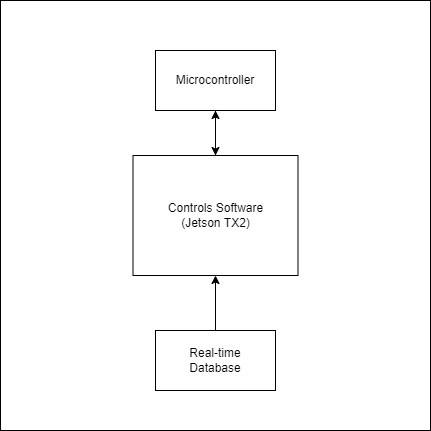
\includegraphics[width=0.60\textwidth]{images/Controls Software Subsystem.drawio.png}
 \caption{Example subsystem description diagram}
\end{figure}

\subsubsection{Assumptions}
The user of the Turning Board is assumed to always be connected to a network (To allow them to access the World Wide Web) to ensure that data can be received from the database and forwarded to the wheels.

\subsubsection{Responsibilities}
After fetching data from the database, the controls software will process the data first to an extent. Since data coming in will be floating point values, it first needs to be translated into value which the microcontroller can understand. So, the entire range of data from the remote control app is taken and the required data is mapped from 0-255 which is then forwarded to the microcontroller which causes the wheels to change speed. As part of the same data packet, angle data from the controls code is also sent to the microcontroller which aids in turning the turning mechanism to a specific angle with respect to the turning mechanisms origin. Any data such as weight values if someone is standing on the long board (an integral part of the design so that the software knows when to turn off the turning mechanism) is received back in the same data format (0-255) which gets translated to weight values inside of the controls code.

\subsubsection{Subsystem Interfaces}
Each of the inputs and outputs for the subsystem are defined here.

\begin {table}[H]
\caption {Controls Software Interfaces} 
\begin{center}
    \begin{tabular}{ | p{1cm} | p{5cm} | p{3cm} | p{5cm} |}
    \hline
    ID & Description & Inputs & Outputs \\ \hline
    \#1 & Data Fetching \& Wheel Velocity Control & \pbox{3cm}{Speed value} & \pbox{5cm}{Change wheel velocity}  \\ \hline
    \#2 & Controlling turning mechanism & \pbox{3cm}{Angle value \\ Weight Value} & \pbox{5cm}{Rotates the turning mechanism \\ Toggles turning mechanism (on/off)}  \\ \hline
    \end{tabular}
\end{center}
\end{table}
